349. Раз Виктор проиграл Георгию четверть игр между ними, всего было 4 игры, 3 из которых он выиграл, то есть игры Виктора и Георгия закончились со счётом $3:1,$ а Георгия и Виктора --- $1:3.$ Алексей проиграл Борису 2 раза, значит и всем остальным он проиграл по 2 раза, и игры Виктора и Алексея закончились со счётом $2:3,$ Алексея и Виктора $3:2,$ Алексея и Бориса $1:2,$ Бориса и Алексея $2:1.$ Из таблицы определим, что Георгий проиграл Борису 2 раза, а выиграл у него 0 раз, значит игры Бориса и Георгия закончились со счётом $2:0,$ а Георгия и Бориса со счётом $0:2.$ Борис выиграл 5 раз, значит игры Бориса и Виктора закончились со счётом $1:7,$ а Виктора и Бориса --- $7:1.$ Георгий выиграл 3 раза, значит проиграл он 9 раз, и игры Алексея и Георгия закончились со счётом $4:2,$ а Георгия и Алексея --- $2:4.$ Таким образом, таблица полностью заполнена.
\begin{figure}[ht!]
\center{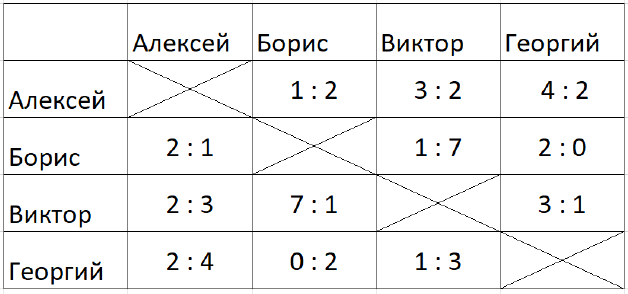
\includegraphics[scale=0.35]{tab2.png}}
\end{figure}\\
